\documentclass{report}
\usepackage[utf8]{inputenc}
\usepackage{amsmath, amssymb}
\usepackage{graphicx}
\usepackage[margin=1.25in]{geometry}
\usepackage{multirow}
\usepackage{pdfpages}
\usepackage{float}
\usepackage{hyperref}
\hypersetup{
    colorlinks,
    citecolor=black,
    filecolor=black,
    linkcolor=black,
    urlcolor=black
}
\title{Lab \#4: Geometrical Optics}
\author{Neil Sawhney}
\date{November 2021}

\makeatletter
\def\@makechapterhead#1{%
  \vspace*{50\p@}% <----------------- Space from top of page to Chapter #
  {\parindent \z@ \raggedright \normalfont
    \ifnum \c@secnumdepth >\m@ne
        \huge\bfseries \thechapter.\ % <-- Chapter # (without "Chapter")
    \fi
    \interlinepenalty\@M
    #1\par\nobreak% <------------------ Chapter title
    \vskip 40\p@% <------------------ Space between chapter title and first paragraph
  }}
\makeatother
\begin{document}

\includepdf[pages=-]{Ph291_Lab4_Cover.pdf}

\maketitle
\tableofcontents

\chapter{Purpose}
The objective of the experiment was to determine the focal length of a lens using Bessel's method. To verify the results, Bessel's method was repeated for two lenses of different focal lengths, which were used to construct a simple telescope. The expected magnification of the telescope was then compared to the observed magnification.
%-----------------------------------

\chapter{Data}

\begin{table}[H]
    \centering
    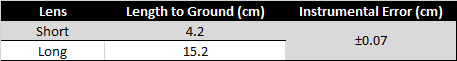
\includegraphics{approxFocalLengths.png}
    \caption{Approximate Focal Lengths}
    \label{approxFocalLengths}
\end{table}
\bigskip

\begin{table}[H]
    \centering
    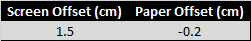
\includegraphics{offsets.png}
    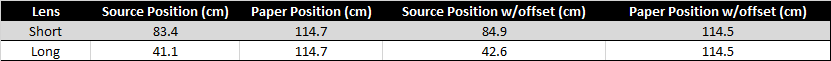
\includegraphics[width = \textwidth]{offsetPositions.png}
    \caption{Source and paper positions after accounting for offsets}
\end{table}
\bigskip

\begin{table}[H]
    \centering
    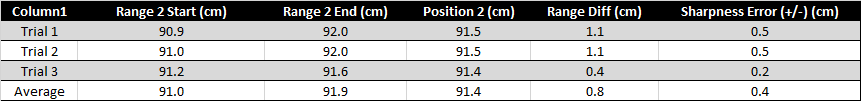
\includegraphics[width = \textwidth]{shortLensSharpnessError.png}
    \caption{Short lens sharpness error}
    \label{shortLensSharpnessError}
\end{table}
\bigskip

\begin{table}[H]
    \centering
    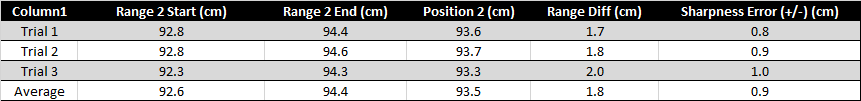
\includegraphics[width = \textwidth]{longLensSharpnessError.png}
    \caption{Long lens sharpness error}
    \label{longLensSharpnessError}
\end{table}

\begin{table}[H]
    \centering
    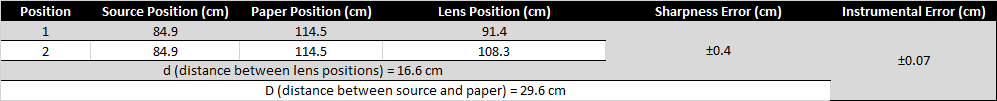
\includegraphics[width = \textwidth]{shortLensPositions.png}
    \caption{Positions for the short lens}
    \label{shortLensPositions}
\end{table}
\bigskip

\begin{table}[H]
    \centering
    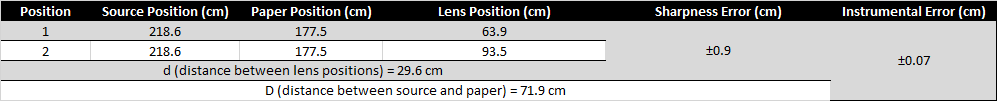
\includegraphics[width = \textwidth]{longLensPositions.png}
    \caption{Positions for the long lens}
    \label{longLensPositions}
\end{table}
\bigskip

\begin{table}[H]
    \centering
    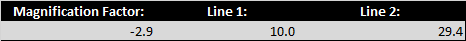
\includegraphics[width = \textwidth]{telescopeTest.png}
    \caption{Length of lines for telescope test}
    \label{telescopeTest}
\end{table}
\bigskip



\chapter{Sources of uncertainty}
One source of uncertainty is the accuracy in determining the difference in length between the non magnified longer line, and the magnified shorter line while looking through the telescope.
A second source of uncertainty is the accuracy in determining the boundaries of when the image is sharp and not sharp.
A third source of uncertainty is the use of the thin lens approximation in the calculations.
A fourth source of uncertainty is the difficulty in reading the linear scale affixed to the optical bench.


\chapter{Calculations}



\section{Derivation for Focal Length}

\label{question1}
$$
    D=2p+d          \hspace{2em}
    D=2i-d         \hspace{2em}
    p=\frac{D-d}{2} \hspace{2em}
    i=\frac{D+d}{2} \hspace{2em}
$$

\begin{equation}
    \frac{1}{f} =\frac{1}{p}+\frac{1}{i}
    \label{thinLensFormula}
\end{equation}

{\scriptsize f = focal length; p = source distance; i = image distance}

$$
    \begin{aligned}
        \frac{1}{f} & =\frac{2}{D-d}+\frac{2}{D+d}      \\
        \frac{1}{f} & =\frac{2(D+d)+2(D-d)}{(D+d)(D-d)} \\
        f           & =\frac{(D+d)(D-d)}{2(D+d)+2(D-d)} \\
        f           & =\frac{(D+d)(D-d)}{4 D}
    \end{aligned}
$$

\begin{equation}
    f =\frac{D^{2}-d^{2}}{4 D}
    \label{focalLength}
\end{equation}

If we solve for d, we get

$$
    \begin{aligned}
        f               & =\frac{D^{2}-d^{2}}{4 D} \\
        4 f             & =D-\frac{d^{2}}{D}       \\
        \frac{d^{2}}{D} & =D-4 f                   \\
        d^{2}           & =D(D-4 f)                \\
        d               & =\sqrt{D(D-4 f)}
    \end{aligned}
$$

It's clear now that if D $<$ 4f, d will have complex solutions which, for this example have no meaning in the real world.

\section{Focal Length}


After plugging in values from \ref{shortLensPositions} into \ref{focalLength},

$$
    \begin{aligned}
        f & =\frac{29.6^{2}-16.6^{2}}{4*29.6} \\
          & =\frac{600.6}{118.4}              \\
          & =5.07
    \end{aligned}
$$

\subsection{Error Propagation for Focal Length from \ref{shortLensPositions}}
$$
    \begin{aligned}
        \delta f & =\sqrt{\left(\frac{\partial f}{\partial D} * \delta D\right)^2+\left(\frac{\partial f}{\partial d} * \delta d\right)^2} \\
                 & =\sqrt{\left(\frac{D^{2}+d^{2}}{4 D^{2}} * \delta D\right)^2+\left(-\frac{d}{2 D} * \delta d\right)^2}                  \\
                 & =\sqrt{\left(\frac{(29.6)^{2}+(16.6)^{2}}{4(29.6)^{2}} * 0.07\right)^2+\left(\frac{-(16.6)}{2(29.6)} * 0.4\right)^2}    \\
                 & =0.11 \mathrm{cm}
    \end{aligned}
$$



\section{Angular Magnification}

$$
    m_{\theta} =-\frac{f_{o}}{f_{e}}
$$
{\scriptsize $f_o$ = Focal length of the objective lens (The long lens); $f_e$ = Focal length of the eye lens (The short lens)}
$$
    \begin{aligned}
        m_{\theta} & =-\frac{14.9}{5.1} \\
                   & =-2.92
    \end{aligned}
$$

\subsection{Error Propagation for Magnification}
$$
    \begin{aligned}
        \delta \mathbf{m}_{\theta} & =\sqrt{\left(\frac{\partial m_{\theta}}{\partial f_{\text {obj }}} * \delta f_{\text {obj }}\right)^{2}+\left(\frac{\partial m_{\theta}}{\partial f_{\text {eye }}} * \delta f_{\text {eye }}\right)^{2}} \\
                                   & =\sqrt{\left(-\frac{1}{f_{\text {eye }}} * 0.2\right)^{2}+\left(\frac{f_{\text {obj }}}{f_{\text {eye }}} * 0.1\right)^{2}}                                                                         \\
                                   & =\sqrt{\left(\frac{1}{5.1} * 0.2\right)^{2}+\left(\frac{14.9}{5.1^{2}} * 0.1\right)^{2}}                                                                                                                \\
                                   & =0.069 
    \end{aligned}
$$



\section{Calculations used in data tables}
\subsection{Sharpness error}
Used in Tables \ref{shortLensSharpnessError}, \ref{longLensSharpnessError}
$$
\text{Sharpness Error} = \frac{\text{Range Diff}}{2}
$$

\subsection{Error Propagation for Linear Scale}
Used in Tables \ref{approxFocalLengths}, \ref{shortLensPositions}, \ref{longLensPositions}
$$
    \begin{aligned}
        \delta \mathbf{D} & =\sqrt{(0.05)^{2}+\left(0.05^{2}\right)} \\
                          & =0.07 \mathrm{~cm}
    \end{aligned}
$$

\subsection{Focal Length Approximations}

\label{question2}
Used in Tables \ref{approxFocalLengths}
\newline
\newline
The distance from the lens to the source was approximated to be infinite, since the distance from the lens to the ceiling was significantly larger than the focal length of the lens. Using this approximation, the approximate focal length of the lens is just the distance between the lens and the floor. \\
\newline
The logic behind this approximation is shown below, starting with the thin lens equation from \ref{thinLensFormula}

$$
    \frac{1}{f} = \frac{1}{p} + \frac{1}{i}
$$

If p $>>$ f, then we can take the limit as u goes to infinity.

$$
    \begin{aligned}
        \lim_{p\to\infty}(\frac{1}{f}) & = \lim_{p\to\infty}(\frac{1}{p} + \frac{1}{i}) \\
        \frac{1}{f}                    & = \frac{1}{i}                                  \\
        f                              & = i
    \end{aligned}
$$
\\
Because the source distance is not infinite, this approximation will slightly overestimate the value of f.




\chapter{Results}


\section*{Focal lengths of lenses}

\begin{equation*}
    \begin{aligned}
        \text{Short Lens} & = 5.1 \pm 0.1 \ \mathrm{cm} \\
        \text{Long Lens}  & = 14.9 \pm 0.2 \ \mathrm{cm}\\
    \end{aligned}
\end{equation*}


\section*{Angular magnification of lenses}

\begin{equation*}
    \begin{aligned}
        \text{Calculated angular magnification factor}   & = -2.92 \pm 0.07  \\
    \end{aligned}
\end{equation*}

The smaller line, whose length is presented in Table \ref{telescopeTest} appeared roughly the same size as the longer line when viewed through the telescope.




\chapter{Conclusions}



The short lens had a calculated focal length of 5.1 ± 0.1 cm, while as the long lens had a calculated focal length of 14.9 ± 0.2 cm. 
The approximation for the focal length of the short lens was 4.2 cm ± 0.07 cm while as the approximation for the long lens was 15.2 ± 0.07 cm. Both calculated values are not within the error bounds of the approximation. This suggests that a source of error has not been properly accounted for.

The approximation that the distance to the source is infinite shown in \ref{question2} is likely not the main culprit, because it would result in an overestimate of the approximation, while as the short lens was underestimated by 0.9 cm. It is possible that the thin lens approximation, or the difficulty in determining the bounds in which the image is sharp, played the more significant role.

In the experimental method, the smaller line, whose length is presented in Table \ref{telescopeTest} appeared roughly the same size as the longer line when viewed through the telescope. This implies the error associated with the experimental method was greater than the error of the original approximation.




\chapter{Answered Questions}



Click under each question to be brought to the location where the respective question is answered.

\section{Question 1}
\hyperref[question1]{Derivation for focal length}

\section{Question 2}
\hyperref[question2]{Focal length approximation}

\end{document}
